Dans ce chapitre, nous présenterons une autre étude de l'interaction entre un utilisateur et un agent virtuel dans le contexte d'une négociation collaborative. 
Notre objectif est d'étudier l'influence de la relation de dominance sur le processus de négociation. Nous nous intéressons à l'impact de la complémentarité de la dominance sur l'augmentation du gain commun dans la négociation et à l'appréciation du partenaire durant la négociation.

En premier lieu, les objectifs généraux de cette étude seront présentés (section \ref{sec:obj}). Nous détaillerons la méthodologie employée pour le paramétrage des agents utilisés dans cette expérimentation (section \ref{sec:methodo}) ainsi que les hypothèses que nous formulons (section \ref{sec:H}).

Nous présenterons ensuite le protocole expérimental employé (section \ref{sec:procedure}). Enfin, nous décrirons les résultats obtenus  (section \ref{sec:res})
que nous discuterons ensuite \ref{sec:discussion}
\section{Objectif}
\label{sec:obj}

Des études en psychologie sociale qui ont exploré l'impact de la relation de dominance sur l'expérience de la négociation et de ses résultats. Certains travaux ont montré l'impact de la complémentarité de la dominance tant sur le vécu de la négociation que sur les résultats obtenues en fin de négociation.
En parallèle, d'autres travaux ont étudié l'impact de la mimicrie ou bien la similarité dans les comportements de dominance dans la négociation. Les résultats obtenus ont démontré leurs impact positif sur la négociation.

Partant de ces études, notre objectif est d'explorer l'impact de ces comportements de dominance qu'ils soient complémentaires ou similaires sur les stratégies de négociation dans le contexte d'une négociation collaborative entre un agent et un utilisateur. Cependant, comme la relation de dominance qui s'installe durant l'interaction est forcément complémentaire nous pensons que les stratégies complémentaires auront un impact positif plus important que des stratégies similaires.
% Ceci nous motive à adapter les hypothèses présentées dans les recherches en psychologie sociale à notre étude. Nous présenterons dans la section suivante les hypothèses que nous avons formulé sur l'impact de la relation complémentaire de dominance sur la négociation.

\subsection{Complémentarité Vs mimicrie en psychologie sociale}
	Reprendre les différentes théories et les principaux résultats obtenue
	
	\subsubsection{Résultats}
		Meilleur gain commun
		Appréciation
		... 
		
\section{Méthodologie}
\label{sec:methodo}

	Afin d'illustrer notre modèle de négociation, nous reprenons le scénario d'une négociation collaborative pour le choix d'un restaurant.
	Ce scénario ne nécessite aucune une expertise pour prendre part dans la négociation. De plus, il est facile pour les participants de reporter leur préférences pour les différents critères pris en compte pour le choix d'un restaurant. En effet, nous considérons les critères \textit{cuisine, ambiance, localisation et prix} pour le choix d'un restaurant, chaque critère est défini avec un ensemble de valeurs présenté dans la table \ref{tab:valeursCritere}. Un total de 630 options ont été généré à partir des critère regroupant les différentes possibilités.
	
	Trois paramètres importants sont à prendre en compte pour initialiser les comportements des agents. 
	En premier lieu, fixer la valeur initiale de pouvoir affectée à chaque agent, nous avons choisi une valeur de pouvoir $pow =0.55$ afin d'avoir un comportement de pouvoir initialement neutre.
	
	En second lieu, il faut initialiser les préférences des agents. Afin d'éviter les limites rencontrées dans la précédente étude, nous avons demandé aux participants de saisir leur préférences (voir section \ref{sec:procedure}).
	
	A partir des préférences saisies par le participant, nous générons automatiquement les préférences des agents suivant certaines conditions.
	La première condition visait à générer des modèles de préférences différents de celui communiqué par l'utilisateur dans le but de créer une confrontation qui pousse à la négociation. Pour cela, nous avons utilisé la distance de kendall \cite{bra2013Kendall}  (\emph{Kendall's  $ \tau \in [0,1]$}) afin de définir la limite minimale de différence entre le modèle de l'agent et celui de l'utilisateur. Par conséquent, nous avons fixer la distance à (\emph{Kendall's  $ \tau \geq 0.7$}).
	
	La seconde condition assurait la différence entre les modèles de préférences générées pour les différents agents. 
	Notre objectif est d'éviter une forte ressemblance entre les préférences des agents due à la première condition. Par conséquent, les agents peuvent donner l'impression d'interagir avec la même entité qui exprime différents comportements. 
	
	Nous avons donc garder uniquement des modèles différents (Kendall's  $ \tau \geq 0.35$). De plus, nous avons ajouté une condition qui assure une différence de perception. pour chaque critère, les modèles ne devaient pas avoir les mêmes valeurs en top des préférences. 
	
	Par exemple, deux modèles \emph{P1, P2} dont la distance est supérieur à $0.35$. De plus, pour le critère \textit{cuisine}, les deux modèles ont la valeur $Italien$ comme la valeur la plus satisfiable $sat_{P1}(Italien) = 1$ et $sat_{P2}(Italien) = 1$. Ces deux modèles sont automatiquement rejetés.
	
	En dernier lieu, nous avons paramétré la stratégie comportemental des agent. Comme note but est d'analyser l'impact de la complémentarité versus la similarité durant la négociation, nous avons implémenté trois stratégies distinctes reproduisant les comportements désirés. 
	A partir de notre algorithme de la théorie de l'esprit, l'agent calcule la valeur de pouvoir de l'utilisateur $pow_{user}$ pour chaque tour de parole exprimé par ce dernier. Suivant la valeur de pouvoir calculée $pow_{user}$, l'agent adopte une des stratégie suivante:
	
	
%	Nous avons implémenté trois agents, tous initialisé avec une valeur de pouvoir
%	De plus, chaque agent adopte une stratégie distincte représentant une condition expérimentale pour notre étude: 
	
	\begin{enumerate}
		\item \textit{Comportement complémentaire}: L'agent adopte un comportement de pouvoir complémentaire à celui exprimé par son partenaire $pow_{agent}=1-pow_{user}$.
		
		\item \textit{Comportement similaire}: L'agent va adopter une stratégie similaire à celle exprimé par son partenaire. C'est à dire que l'agent va imiter les comportements de pouvoir exprimé par le participant $pow_{agent} = pow_{user}$.
		
		\item \textit{Comportement de contrôle} : L'agent ne s'adapte pas à son interlocuteur et suit un comportement de pouvoir statique.
	\end{enumerate}
	
	En modifiant la valeur de pouvoir de l'agent à chaque tour, nous avons du ajouter une contrainte dans son le modèle décisionnel de l'agent afin d'assurer une cohérence des les comportements générés. 
	En effet, la valeur de pouvoir est essentielle pour le calcul des satisfiabilité des valeurs et un changement de cette valeur risque de fausser les préférences de l'agent.
	Par exemple, à un moment $t$ de la négociation, une valeur $v$ est satisfiable, mais due à une adaptation qui cause un changement de pouvoir la même valeur $v$ peut devenir non satisfiable.
	En vue de protéger des préférences et donc la cohérence des comportements de l'agent, nous avons fait le choix d'utiliser uniquement la valeur de pouvoir initiale $pow_{agent} = 0.55$ pour calculer la satisfiabilité des valeurs.
	
	Nous avons donc implémenté trois agents \emph{Bob, Arthur} et \emph{Kevin}. \emph{Bob} adoptant un comportement complémentaire, \emph{Arthur} qui suit un comportement similaire à celui exprimé par son partenaire de négociation, et enfin \emph{Kevin}, un agent contrôle qui suit une seul stratégie de pouvoir neutre. 
	
\section{Hypothèses}
\label{sec:H}

	suivant les travaux de \cite{}, nous supposons que la relation de dominance établie entre l'agent et l'utilisateur a une influence sur les stratégies exprimées par les négociateurs. Elle va donc avoir une conséquence sur les résultats obtenues lors de la négociation ainsi que l'appréciation que les négociateurs ont ressentis en négociant avec leur partenaire. Par conséquent, nous définissons les hypothèses suivantes: 
		\begin{itemize}
			\item [$\bullet$] \textbf{H1}: Les négociateurs atteignent un gain commun plus important quand les négociateurs établissent une relation de dominance complémentaire.
			\item [$\bullet$] \textbf{H2}: La négociation converge plus rapidement dans le cas où les négociateurs ont un relation de dominance complémentaire. 
			\item [$\bullet$] \textbf{H3}: Le négociateur se sent plus à l'aise avec un partenaire qui exprime un comportement complémentaire.
			\item [$\bullet$] \textbf{H4}: La complémentarité dans la relation de dominance augmente l'appréciation entre les négociateurs.
		\end{itemize}



\section{Protocole expérimentale}
\label{sec:procedure}
	Nous présentons dans cette section, le protocole expérimental employé, en commençant par les mesures utilisés pour questionner les participants sur leur interactions. Ensuite, nous présenterons la population de participants et enfin le protocole suivi pour chaque participant. 
	
	\subsection{Mesures}
		Après chaque interaction avec un agent, le participant était invité à remplir un questionnaire abordant trois points principaux. De plus, pour chaque questionnaire, nous avons insérés quelques items de manipulations afin de vérifier la concordance des réponses. 
		
		\subsubsection{Questionnaire en auto-attribution} Les participants ont répondu pour eux-même au questionnaire des comportements de pouvoir dans la négociation que nous avons conçu, afin de mesurer les comportements qu'ils ont exhibé durant leur interaction. Ce questionnaire utilise une échelle de Likert à 5 points. Nous présentons ci-dessous les items de ce questionnaire. 
		\begin{enumerate}
				\item J'ai été égocentrique pendant la négociation
				\item J'ai pris en compte les préférences de l'agent.
				\item J'ai été exigeant(e).
				\item J'ai maintenu ma position durant la négociation.
				\item J'ai abandonné ma position durant la négociation
				\item J'ai fait des concessions pendant la négociation.	
				\item J'ai mené la négociation.
				\item J'étais leader dans la négociation
		\end{enumerate}
		 
		 \subsubsection{Questionnaire en hétéro-attribution}
		 Les participants ont répondu à un questionnaire afin de décrire leur perception de l’agent avec lequel ils interagissaient.
		 
		 Nous nous sommes principalement intéressés aux comportements de pouvoir exprimés par l'agent. Pour cela, nous avons utilisé le même questionnaire sur les comportements de pouvoir (voir section ...)
 
		 \subsection{Questionnaire concernant l'interaction}
		 Pour évaluer l'appréciation du participant vis a vis de l'interaction qu'il a eu avec l'agent. Nous nous sommes basés sur les travaux de \cite{tiedens2003power} pour définir le questionnaire ci-dessous:
		
		 \begin{enumerate}
		 	\item Je suis satisfait de la décision finale.
		 	\item La décision finale était équitable pour nous deux.
			\item Je me suis senti à l'aise pendant la négociation.
			\item J'ai trouvé que la négociation avec l'agent était aisée.
			\item Je me sentais détendu pendant la négociation.
			\item Je me sentais anxieux pendant la négociation.
			\item J'ai apprécié la négociation avec l'agent.
		 \end{enumerate}
		 
		  \subsection{Données d'interactions}
		  Nous avons enregistré les informations suivantes à chaque interaction
		  \begin{itemize}
		  	\item Les préférences du participant et celles de l'agent.
		  	\item Les tours de paroles avant de trouver un compromis
		  	\item Le pouvoir du participant calculé à partir de l'algorithme de théorie de l'esprit après chaque tour de parole.
		  	\item Le dialogue généré.
		  	
		  \end{itemize}


	\subsection{Protocole}
		Après avoir expliqué le but de l'étude qui portait sur l'évaluation des comportements d'agents virtuels. L'expérimentateur développait le déroulé de l'étude. 
		Premièrement, il expliquait que le but de l'interaction était de négocier avec chaque agent afin de trouver un restaurant où aller dîner. Il leur donnait des instructions afin de se projeter dans une situation réelle en plus de mettre l'accent sur l'aspect "collaboratif" de la négociation comme présenté dans la figure \ref{fig:instruction}.
		
		\begin{figure}[h]
			\fbox{\begin{minipage}{.95\textwidth}
					{\ttfamily
					\textbf{Instruction:} Mettez vous dans la situation où vous allez dîner avec un ami ou un collègue pour la première fois, vous ne connaissez pas ses préférences et il ne connaît pas les votres. Le but est de négocier en fonction de vos préférences respectives pour de choisir un restaurant qui \underline{vous convienne à tous les deux}.
					}
				\end{minipage}}
				
				\caption{\label{fig:instruction}Excerpt of Dialogue 2.}
			\end{figure}


		Une fois le but de l'étude expliqué, l'expérimentateur lançait la phase de tutoriel afin de familiariser le participant à l'utilisation de l'interface de communication. 	L'expérimentateur présentait les différents les actes de dialogues possibles pour communiquer avec l'agent. 	
		Le participant était informé que durant cette session l'agent ne répondait pas à ses actes, et que le but était de manipuler l'interface pour générer des actes. 
	
		L’expérimentateur répondait alors à d’éventuelles questions concernant la génération d'actes de dialogue ou leur significations.
		
		Ensuite, l’expérimentateur annonçait au participant qu’il/elle allait négocier avec trois différents agents virtuels et
		qu’après chaque négociation, il/elle devrait répondre à différents questionnaires pour évaluer son interaction avec l’agent avec lequel il/elle
		venait de négocier.  Avant de commencer l'expérience, le participant est invité à saisir ses préférences pour les valeurs de chaque critères dans un ordre décroissant (voir la figure \ref{fig:pref}).
		
		Une fois les préférences pour les différentes valeurs de critères saisies, la fenêtre avec le premier agent s'ouvrait automatiquement invitant le participant à prendre part à la négociation. 
		
		\begin{figure}[b]
			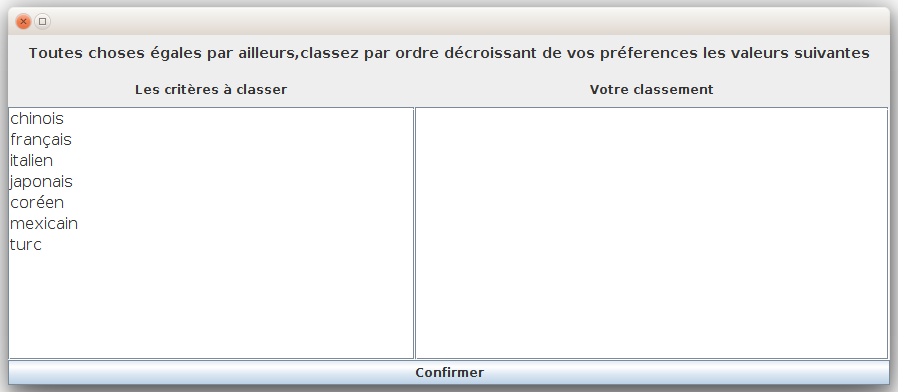
\includegraphics[width=4in]{Figures/pref.png}
			\caption{\label{fig:pref} Interface pour la saisie d'ordre de préférence. Exemple pour le critère de cuisine}
		\end{figure} 

		

\section{Résultats}
\label{sec:res}
Nous avons mené une étude intra-sujet dans laquelle 63 participants ont pris part.  Cependant deux participants ont été écarté car ils ne remplissaient pas les conditions (mauvaise réponse à la majorité des questions de manipulations). 
Notre étude statistique a été mené sur les 61 participants restants. 	

Nous avons d'abord analyser la perception des comportements de pouvoir lors de la négociation. En effet, avant d'analyser les hypothèses, nous voudrions étudier la perception des stratégies de complémentarité et la similarité durant la négociation.

Plan des résultats 
\begin{itemize}
	\item comportement de pouvoir
	\item Gain commun
	\subitem Gain commun en perceptif
	\item tour de parole pour appuyer le gain
	\subitem Négociation aisée 
	\item Appréciation
	\item Confort
	\item Proposition complémenter les test en gardant que les participants ayant perçu complémentarité Vs similarité pour la perception de l'appréciation
	
\end{itemize}

\section{Discussion}
\label{sec:discussion}